\subsection{Experimental Setup}
\label{subsec:experimental-setup}

% Experiments
We evaluate our approach using two real-world bioinformatics workflows: \textit{rnaseq-star-deseq2}\footnote{\url{https://github.com/snakemake-workflows/rna-seq-star-deseq2}}, which aligns RNA sequencing reads and computes differential gene expression (135 jobs), and \textit{stained glass}\footnote{\url{https://github.com/mrvollger/StainedGlass}}, which computes sequence-identity heatmaps of genome assemblies (44 jobs). Per workflow, we run PEFO as baseline and LJF and SISF with two time-to-result targets each (310 and 250\,min for rnaseq-star-deseq2, 75 and 65\,min for stained glass).

Table~\ref{tab:results} reports the number of offloaded jobs $|J_\mathrm{off}|$, the prediction error (PE) of the predicted makespan relative to the observed median makespan, whether the time-to-result target was met, and the change in makespan and offloading cost relative to PEFO.
We derive costs from the runtime and the requested vCPUs, memory, and ephemeral storage of each offloaded job, priced at on-demand Google Kubernetes Engine (GKE) Autopilot rates\footnote{\url{https://cloud.google.com/kubernetes-engine/pricing}} as a reference for a commercial secondary environment.

% Infrastructure 
We use two Kubernetes clusters, each with two nodes (AMD EPYC 7282, 32 threads, 125 GiB RAM, 3.5 TB SSD), connected at 5 Gbit/s to emulate geo-distributed links.

\subsection{Experimental Results}
\label{subsec:experimental-results}
Makespan prediction with the Bayesian median ($q=0.5$) achieves a MAPE of 6.0\,\% for LJF and SISF and 6.4\,\% for PEFO. LJF deviates by at most 3.3\,\%, whereas SISF overestimates the makespan of rnaseq-star-deseq2 by 11.3\,\% and 17.4\,\%.
Overestimation is uncritical for the time-to-result, as both SISF runs still finish 35 and 37\,min early. Underestimation is not, as LJF with the 250\,min target of rnaseq-star-deseq2 misses it by 6\,min at a prediction error of only $-2.3$\,\%. All other experiments meet their target.
Offloading once the primary cluster runs out of resources (PEFO) shortens the makespan by 36.5\,\% for rnaseq-star-deseq2 and 31.0\,\% for stained glass, but also incurs the highest offloading cost. LJF and SISF trade part of this speed-up for cost and reduce the offloading cost by 40.6\,\% compared to PEFO at a 14.8\,\% longer makespan. For the 310\,min target of rnaseq-star-deseq2, LJF offloads only five jobs and lowers the cost from \$5.58 to \$2.07. Cost depends on the runtime and resources of the offloaded jobs rather than their number, as SISF with 35 jobs is cheaper than LJF with five for the 310\,min target. With the 250\,min target, SISF even outperforms PEFO in both makespan and cost.

\begin{figure}[t]
    \centering
    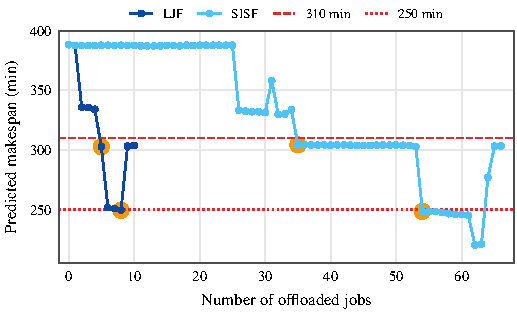
\includegraphics[width=\columnwidth]{img/evaluation/workflow_offloading_steps_rna-seq-star-deseq2.pdf}
    \caption{Bayesian predicted makespan after each offloading step for rnaseq-star-deseq2. Circles mark the job sets selected for each time-to-result target.}
    \label{fig:makespan-offloading-dependence}
\end{figure}

% Results Table
\begin{table}[t]
\caption{Makespan prediction error (PE) and change in median makespan ($\Delta$M) and offloading cost ($\Delta$C) relative to PEFO (\checkmark/$\times$: time-to-result met/missed).}
\label{tab:results}
\centering
\footnotesize
\setlength{\tabcolsep}{3pt}
\begin{tabular}{llrrrr}
\hline
\textbf{Workflow} & \textbf{Criterion ($C$)} & $|J_\mathrm{off}|$ & \textbf{PE} & $\Delta$\textbf{M} & $\Delta$\textbf{C} \\
\hline
rnaseq-star- & LJF (310\,min) \checkmark & 5 & +3.3\,\% & +29.8\,\% & $-$62.8\,\% \\
deseq2 & LJF (250\,min) $\times$ & 8 & $-$2.3\,\% & +12.7\,\% & $-$30.0\,\% \\
 & SISF (310\,min) \checkmark & 35 & +11.3\,\% & +21.2\,\% & $-$65.0\,\% \\
 & SISF (250\,min) \checkmark & 54 & +17.4\,\% & $-$6.3\,\% & $-$3.1\,\% \\
stained glass & LJF/SISF (75\,min) \checkmark & 2 & +1.1\,\% & +28.5\,\% & $-$70.4\,\% \\
 & LJF/SISF (65\,min) \checkmark & 6 & $-$0.8\,\% & +8.7\,\% & $-$20.4\,\% \\
\hline
\end{tabular}
\end{table}

% Makespan vs. Offloading
How many jobs are needed depends on the selection criterion, as Fig.~\ref{fig:makespan-offloading-dependence} shows for rnaseq-star-deseq2. Offloading the longest jobs first lowers the makespan right away, so LJF meets the 310\,min target after five jobs. SISF first offloads jobs with small inputs, so its prediction stays nearly constant from the second to the 25th job and it needs 26 jobs for the same target.

% Discussion
Our results show that simulating the makespan before execution lets SOU offload only as many jobs as a given time-to-result requires. Although most targets are met, the single miss occurs when the predicted makespan lies very close to the target. The time-to-result should therefore be understood as a soft constraint, as SOU selects a configuration that is predicted, but not guaranteed, to meet it. Moreover, offloading additional jobs does not always shorten the predicted makespan further (Fig.~\ref{fig:makespan-offloading-dependence}), which shows that the choice of jobs matters more than their number. 
Remaining prediction errors mainly stem from three sources. Runtimes vary under resource contention, tasks whose runtime does not correlate with input size fall back to the median runtime, and the simulation does not yet model job retries.